\documentclass[11pt]{article}
\usepackage[a4paper,margin=2.5cm]{geometry}
\usepackage[T1]{fontenc}
\usepackage[utf8]{inputenc}
\usepackage{lmodern}
\usepackage{microtype}
\usepackage{graphicx}
\usepackage{booktabs}
\usepackage{tabularx}
\usepackage{array}
\usepackage{amsmath}
\usepackage[numbers,sort&compress]{natbib}
\usepackage{xcolor}
\usepackage{float}
\usepackage{xurl}
\usepackage[colorlinks=true,linkcolor=blue!50!black,citecolor=blue!50!black,urlcolor=blue!50!black]{hyperref}

\newcommand{\NClaudeRuns}{792}
\newcommand{\NClaudeSessions}{899}
\newcommand{\NLocalRuns}{48}
\newcommand{\NAllRuns}{840}
\newcommand{\NAllSessions}{975}
\newcommand{\NVerifyOk}{773}
\newcommand{\NVerifyHaikuFail}{15}
\newcommand{\NVerifyFail}{19}
\newcommand{\TotalCost}{\$64}
\newcommand{\PoolMissCost}{$-$14\%}
\newcommand{\PoolMissCI}{$-$22\% to $-$5\%}
\newcommand{\PoolMissProse}{17/56}
\newcommand{\PoolMissRules}{0/56}
\newcommand{\PoolLoadedCost}{0\%}
\newcommand{\PoolLoadedCI}{$-$11\% to +12\%}
\newcommand{\PoolLoadedProse}{0/32}
\newcommand{\PoolLoadedRules}{0/32}
\newcommand{\HThreeNoLoop}{47/48}
\newcommand{\HThreeNoLoopCI}{89\% to 100\%}
\newcommand{\HThreeNoPointer}{48/48}
\newcommand{\HThreeNoPointerCI}{93\% to 100\%}
\newcommand{\HThreeFull}{47/48}
\newcommand{\HThreeFullCI}{89\% to 100\%}
\newcommand{\HOneBreaks}{8/48}
\newcommand{\HOneBreaksAgainst}{0/48}
\newcommand{\HOneBreaksP}{0.001}
\newcommand{\HOneCost}{+12\%}
\newcommand{\HOneCI}{0\% to +24\%}
\newcommand{\HOneCostP}{0.024}
\newcommand{\HOneN}{96}
\newcommand{\HTwoBreaks}{0/48}
\newcommand{\HTwoBreaksAgainst}{0/48}
\newcommand{\HTwoBreaksP}{1.000}
\newcommand{\HTwoCost}{+13\%}
\newcommand{\HTwoCI}{+3\% to +24\%}
\newcommand{\HTwoCostP}{0.005}
\newcommand{\HTwoN}{96}
\newcommand{\HFourBreaks}{0/5}
\newcommand{\HFourBreaksAgainst}{0/5}
\newcommand{\HFourBreaksP}{1.000}
\newcommand{\HFourCost}{+9\%}
\newcommand{\HFourCI}{$-$9\% to +30\%}
\newcommand{\HFourCostP}{0.177}
\newcommand{\HFourN}{10}
\newcommand{\HFiveBreaks}{3/16}
\newcommand{\HFiveBreaksAgainst}{0/16}
\newcommand{\HFiveBreaksP}{0.100}
\newcommand{\HFiveCost}{+20\%}
\newcommand{\HFiveCI}{+1\% to +42\%}
\newcommand{\HFiveCostP}{0.016}
\newcommand{\HFiveN}{32}
\newcommand{\HSevenBreaks}{3/32}
\newcommand{\HSevenBreaksAgainst}{0/32}
\newcommand{\HSevenBreaksP}{0.121}
\newcommand{\HSevenCost}{+1\%}
\newcommand{\HSevenCI}{$-$9\% to +13\%}
\newcommand{\HSevenCostP}{0.428}
\newcommand{\HSevenN}{64}
\newcommand{\HNineBreaks}{4/32}
\newcommand{\HNineBreaksAgainst}{0/32}
\newcommand{\HNineBreaksP}{0.056}
\newcommand{\HNineCost}{$-$3\%}
\newcommand{\HNineCI}{$-$12\% to +8\%}
\newcommand{\HNineCostP}{0.691}
\newcommand{\HNineN}{64}
\newcommand{\HElevenBreaks}{0/64}
\newcommand{\HElevenBreaksAgainst}{0/64}
\newcommand{\HElevenBreaksP}{1.000}
\newcommand{\HElevenCost}{+3\%}
\newcommand{\HElevenCI}{$-$19\% to +29\%}
\newcommand{\HElevenCostP}{0.402}
\newcommand{\HElevenN}{128}
\newcommand{\HSixBreaks}{3/16}
\newcommand{\HSixBreaksAgainst}{0/16}
\newcommand{\HSixBreaksP}{0.100}
\newcommand{\HSixCost}{+20\%}
\newcommand{\HSixCI}{+1\% to +42\%}
\newcommand{\HSixCostP}{0.016}
\newcommand{\HSixN}{32}
\newcommand{\HEightBreaks}{3/32}
\newcommand{\HEightBreaksAgainst}{0/32}
\newcommand{\HEightBreaksP}{0.121}
\newcommand{\HEightCost}{+1\%}
\newcommand{\HEightCI}{$-$9\% to +13\%}
\newcommand{\HEightCostP}{0.428}
\newcommand{\HEightN}{64}
\newcommand{\HTenBreaks}{4/32}
\newcommand{\HTenBreaksAgainst}{0/32}
\newcommand{\HTenBreaksP}{0.056}
\newcommand{\HTenCost}{$-$3\%}
\newcommand{\HTenCI}{$-$12\% to +8\%}
\newcommand{\HTenCostP}{0.691}
\newcommand{\HTenN}{64}
\newcommand{\SeqOk}{16}
\newcommand{\SeqPlanned}{48}
\newcommand{\HOneCatchFull}{45}
\newcommand{\HTwoCatchNoPointer}{115}
\newcommand{\PoolFourFiveBreaks}{7/64}
\newcommand{\PoolFourFiveP}{0.007}
\newcommand{\NoneVsProseCost}{+35\%}
\newcommand{\NoneVsProseCI}{+21\% to +50\%}
\newcommand{\TaxCost}{+9\%}
\newcommand{\TaxCI}{$-$7\% to +27\%}
\newcommand{\GenBreaks}{0/48}
\newcommand{\GenCost}{$-$25\%}
\newcommand{\GenCI}{$-$32\% to $-$17\%}
\newcommand{\NLoopRuns}{360}
\newcommand{\NLoopBroken}{0}
\newcommand{\PSixPrimaryRuns}{256}
\newcommand{\PSixLocalRuns}{128}
\newcommand{\PSixLatestRuns}{56}
\newcommand{\PSixRuns}{440}
\newcommand{\NTotalRuns}{1280}
\newcommand{\NTotalSessions}{1532}
\newcommand{\PSixCost}{\$163}
\newcommand{\NTotalCost}{\$227}
\newcommand{\HTwelveProse}{28/128}
\newcommand{\HTwelveRules}{17/128}
\newcommand{\HTwelveP}{0.048}
\newcommand{\HTwelveHolm}{0.095}
\newcommand{\HThirteenCost}{+6\%}
\newcommand{\HThirteenCI}{$-$5\% to +18\%}
\newcommand{\HThirteenP}{0.281}
\newcommand{\HThirteenHolm}{0.281}
\newcommand{\HThirteenTaskCost}{+9\%}
\newcommand{\HThirteenTaskCI}{$-$2\% to +21\%}
\newcommand{\PSixBPProse}{15/64}
\newcommand{\PSixBPRules}{16/64}
\newcommand{\PSixBPP}{0.659}
\newcommand{\PSixFBProse}{13/64}
\newcommand{\PSixFBRules}{1/64}
\newcommand{\PSixFBP}{$<$0.001}
\newcommand{\HFourteenProse}{47/64}
\newcommand{\HFourteenRules}{19/64}
\newcommand{\HFourteenP}{$<$0.001}
\newcommand{\PSixBPCatchRuns}{38/64}
\newcommand{\PSixBPIgnoredRuns}{16}
\newcommand{\PSixBPRoleRuns}{31/31}
\newcommand{\PSixBPRoleTFour}{31/31}
\newcommand{\PSixOpened}{32/64}
\newcommand{\PSixOpenedViol}{4/32}
\newcommand{\PSixNotOpenedViol}{6/32}
\newcommand{\PSixBPCells}{1482}
\newcommand{\PSixBPPrecision}{6/16}
\newcommand{\PSixBPPrecisionCI}{15\% to 65\%}
\newcommand{\PSixBPRecall}{6/28}
\newcommand{\PSixBPRecallCI}{8\% to 41\%}
\newcommand{\PSixFBCells}{120}
\newcommand{\PSixFBPrecision}{13/13}
\newcommand{\PSixFBPrecisionCI}{75\% to 100\%}
\newcommand{\PSixFBRecall}{13/13}
\newcommand{\PSixFBRecallCI}{75\% to 100\%}
\newcommand{\PSixBPFpRole}{10}
\newcommand{\PSixBPFnNoAny}{13}
\newcommand{\PSixBPFnZod}{6}
\newcommand{\PSixBPFnOther}{3}
\newcommand{\PSixLoopFalse}{6/82}
\newcommand{\PSixLoopFalseCI}{3\% to 15\%}
\newcommand{\PSixAfterFalse}{2/170}
\newcommand{\PSixAfterFalseCI}{0\% to 4\%}
\newcommand{\PSixBPConventions}{40}
\newcommand{\PSixBPLOC}{491}
\newcommand{\PSixBPCases}{91}
\newcommand{\PSixFBConventions}{4}
\newcommand{\PSixFBLOC}{151}
\newcommand{\PSixFBCases}{18}
\newcommand{\PSevenRuns}{128}
\newcommand{\NTotalRunsEMSE}{1408}
\newcommand{\NTotalSessionsEMSE}{1691}
\newcommand{\PSevenCost}{\$22}
\newcommand{\HSixteenProse}{31/64}
\newcommand{\HSixteenRules}{0/64}
\newcommand{\HSixteenP}{$<$0.001}
\newcommand{\HSixteenHolm}{$<$0.001}
\newcommand{\HSeventeenCost}{$-$24\%}
\newcommand{\HSeventeenCI}{$-$30\% to $-$18\%}
\newcommand{\HSeventeenP}{1.000}
\newcommand{\HSeventeenHolm}{1.000}
\newcommand{\HSeventeenTaskCost}{$-$1\%}
\newcommand{\HSeventeenTaskCI}{$-$8\% to +7\%}
\newcommand{\PSevenDOneProse}{29/64}
\newcommand{\PSevenDOneP}{$<$0.001}
\newcommand{\PSevenAsCast}{21}
\newcommand{\PSevenManager}{7}
\newcommand{\PSevenHelpers}{1}
\newcommand{\PSevenLoopRuns}{38}
\newcommand{\PSevenIgnoredRuns}{0}
\newcommand{\PSevenProseLeft}{1}
\newcommand{\PSevenTurnsProse}{31.7}
\newcommand{\PSevenTurnsRules}{25.5}
\newcommand{\PSevenVerifyProse}{58/64}
\newcommand{\PSevenVerifyProseCI}{81\% to 96\%}
\newcommand{\PSevenVerifyProseFail}{6}
\newcommand{\PSevenVerifyProseTTwo}{4}
\newcommand{\PSevenVerifyRules}{54/64}
\newcommand{\PSevenVerifyRulesCI}{73\% to 92\%}
\newcommand{\PSevenVerifyRulesFail}{10}
\newcommand{\PSevenVerifyRulesTTwo}{10}

% \input is not expandable inside a tabular, so a rule after it fails; the primitive is.
\makeatletter\let\rows\@@input\makeatother
\emergencystretch=3em
\raggedbottom

\newcommand{\file}[1]{\texttt{#1}}
\newcommand{\arm}[1]{\texttt{#1}}
\newcolumntype{L}{>{\raggedright\arraybackslash}X}

\title{Where Should a Coding Rule Live?\\[0.3em]
\large A Controlled Benchmark of Prose Instructions and Lint Rules for AI Coding Agents}
\author{Clirim Ajeti\\
Independent Researcher, Munich, Germany\\
\href{mailto:clirimajeti@gmail.com}{\texttt{clirimajeti@gmail.com}}}
\date{November 2026}

\begin{document}
\maketitle

\begin{abstract}
\noindent
\textbf{Context.}
Software engineering teams write conventions for AI coding agents in Markdown instruction files such as \file{CLAUDE.md} and \file{AGENTS.md}.
Nothing enforces them: the agent may ignore them, and an always-loaded file costs tokens in every session.
An alternative is a lint rule that runs after every edit and reports violations to the agent.

\smallskip\noindent
\textbf{Objective.}
We ask where a coding rule should live to minimize violations and cost.

\smallskip\noindent
\textbf{Method.}
We present agent-rules-bench, an open-source harness that runs the same task in identical copies of a repository, one per rule placement, and measures violations, cost, turns and functional correctness.
We report \NAllRuns{} headless agent runs (\NAllSessions{} sessions): \NClaudeRuns{} Claude Code runs with Claude Sonnet 5.5 and Haiku 5.5 on projects in Java, Python and TypeScript, and \NLocalRuns{} exploratory runs with the local model Qwen3.6 35B-A3B in pi and Codex.
Four studies were exploratory; for the later ones we pre-registered each analysis plan.

\smallskip\noindent
\textbf{Results.}
Exploratory: when the rule was in prose that the agent could miss, it was violated in 17 of 56 runs (11 in production code); as a lint rule, in none, and runs cost 14\% less (95\% CI: 5\% to 22\%) because no run needed a review fix.
In a short always-loaded file, prose matched lint rules.
Pre-registered: (1)~The feedback loop prevented violations of a rule that no prose stated (\HOneBreaks{} vs.\ \HOneBreaksAgainst, $p=\HOneBreaksP$).
(2)~A one-line pointer in the instruction Markdown file avoided rework (\HTwoCost{} cost without it).
(3)~A 15.7k-token always-loaded file cost 20\% more than lint rules ($p=\HSixCostP$).
(4)~Forty conventions as prose and as lint rules came out even in each test; pooled post hoc over two studies, prose was violated in 7 of 64 runs and lint rules in none.
Functional correctness did not differ.

\smallskip\noindent
\textbf{Conclusions.}
The results suggest: put mechanical and often-missed rules in lint rules with an in-session feedback loop, and keep always-loaded prose short.
\end{abstract}

\section{Introduction}
\label{sec:intro}

Teams state their conventions in repository instruction files, which AI coding agents such as Claude Code, Codex and pi read.
Typical conventions are ``inject a clock instead of calling \texttt{now()}'', ``keep database access out of route handlers'', and ``return success messages only from the API layer''.
These files grow.
A rule can then sit in the middle of long text, or in a linked document that the agent does not open.
The agent then copies the nearby code, and the nearby code often violates the rule.
This is especially true for legacy code.

A second place for a rule is a lint rule.
A linter tool checks the code, not the agent's attention.
If a hook runs the linter after every edit, the agent gets the message while it works, and it can fix the violation in the same session.
Practitioners recommend this approach~\cite{evilmartians2026hooks}, but we found no controlled data on it.
Research on agent context files measures whether the files help at all~\cite{gloaguen2026agentsmd,khatri2026contextfiles}, how their structure changes adherence~\cite{mcmillan2026adherence}, and what they contain~\cite{chatlatanagulchai2025agentreadmes}.
It does not compare prose with lint rules for the same rule.

This paper asks one question:
\emph{where should a coding rule live so that an AI coding agent follows it, and what does each place cost?}
We compare five places: prose in a linked document, prose buried in long documents, prose in the always-loaded file, a lint rule with a feedback loop, and a lint rule with a feedback loop and a one-line pointer.

Our contributions are:
\begin{enumerate}
\item \textbf{agent-rules-bench}, an open harness that runs headless agent sessions against identical repository copies, one copy per setup, and measures rule violations on added lines, cost, turns, review-fix rounds and functional correctness (Section~\ref{sec:method}).
\item \textbf{\NAllRuns{} runs} (\NClaudeRuns{} with Claude Code, \NLocalRuns{} with a local model) on three public projects in three languages, with all setups, prompts, transcripts, diffs and logs published.
\item \textbf{Five pre-registered study plans} that test the parts of the lint setup separately and the cost of always-loaded prose (Section~\ref{sec:results}).
\item \textbf{A practical guideline} for teams that write agent instructions (Section~\ref{sec:discussion}).
\end{enumerate}

\section{Background and Related Work}
\label{sec:related}

\paragraph{Context files for coding agents.}
Claude Code loads \file{CLAUDE.md} from the repository root at session start, and loads \file{CLAUDE.md} files in subdirectories when it reads files there.
Codex and pi load \file{AGENTS.md}.
\citet{chatlatanagulchai2025agentreadmes} analyze what developers write in these files.
\citet{gloaguen2026agentsmd} find that context files do not generally improve task success, and that they raise inference cost by over 20\% on average.
They also report that agents follow the instructions in these files well, and that the files are useful to state non-standard coding practices.
\citet{khatri2026contextfiles} finds, in an ablation with Claude Code and Codex, that the context strategy does not measurably change correctness: the agents fail on implementation skill, not on missing repository knowledge.
\citet{mcmillan2026adherence} varies four structural properties of configuration files (size, instruction position, file architecture and conflicting files) in 1,650 Claude Code sessions, and finds no detectable effect of any of them on adherence.
The largest effect in that study is within the session: adherence tends to fall as the agent generates more code.
All of these studies treat the context file as the only place for instructions.
We add the lint rule as a second place and compare both places for the same rule.

\paragraph{Long context.}
Language models use information in the middle of a long context less reliably than information at its start or end~\cite{liu2024lost}.
For instruction files that the agent loads, however, \citet{mcmillan2026adherence} finds no detectable effect of file size or instruction position.
The rules that we call \emph{buried} face a different risk.
They are in linked documents, and the agent may never open the document, so the rule never enters the context at all.
A long session adds a second risk, because adherence can fall as the session goes on~\cite{mcmillan2026adherence}.
A check that runs after every edit does not depend on how long ago the agent read the rule.

\paragraph{Static analysis.}
Static analysis tools find defects early, but developers often ignore their warnings when the warnings arrive late or include false positives~\cite{johnson2013static,sadowski2018google}.
\citet{sadowski2018google} report that developers act on checks that appear during code review and have a low false-positive rate.
A lint rule that runs after each agent edit can meet both conditions: the warning arrives within seconds of the change, and a rule written for one project convention can be written to have a low false-positive rate.
Its message can also state the fix directly.

\paragraph{Benchmarks.}
SWE-bench~\cite{jimenez2024swebench} measures whether an agent resolves real GitHub issues.
mdarena~\cite{mdarena} compares \file{CLAUDE.md} variants on a repository's merged pull requests, and a token-efficiency benchmark~\cite{peker2026tokeneff} compares Claude Code configurations by cost.
None of these benchmarks measures rule violations, or the cost of fixing them, across different placements of the same rule.

\section{Rule Placements}
\label{sec:setups}

Each study fixes a repository at a pinned commit, a small set of rules, and a set of task prompts.
A task prompt describes only the feature to build.
It never mentions the rules and never asks the agent to follow conventions.
Such a hint would send the agent to the documents in every setup and would hide the difference that we want to measure.

The setups, which we call \emph{arms}, differ only in where the rules live:
\begin{itemize}
\item \arm{prose\_linked}: \file{CLAUDE.md} holds one sentence that links to a short document with the rules.
\item \arm{prose\_buried}: \file{CLAUDE.md} links to 8 or 9 realistic documents (4k to 7k tokens), and each rule is one bullet in the middle of one document.
\item \arm{prose\_loaded}: the rules are in the always-loaded \file{CLAUDE.md}.
\item \arm{rules}: no prose states the rules.
Each rule is a lint rule (ast-grep, ESLint or Ruff).
A feedback loop lints each edited file after every edit and returns the findings to the agent (Figure~\ref{fig:loop}).
A one-line pointer in a folder-level \file{CLAUDE.md} names each design-shaping rule.
\end{itemize}
Two further arms take the \arm{rules} arm apart.
\arm{rule\_only} keeps the lint rules and the loop but removes the pointers.
\arm{pointer\_only} keeps the pointers but removes the loop.

\begin{figure}[H]
\centering
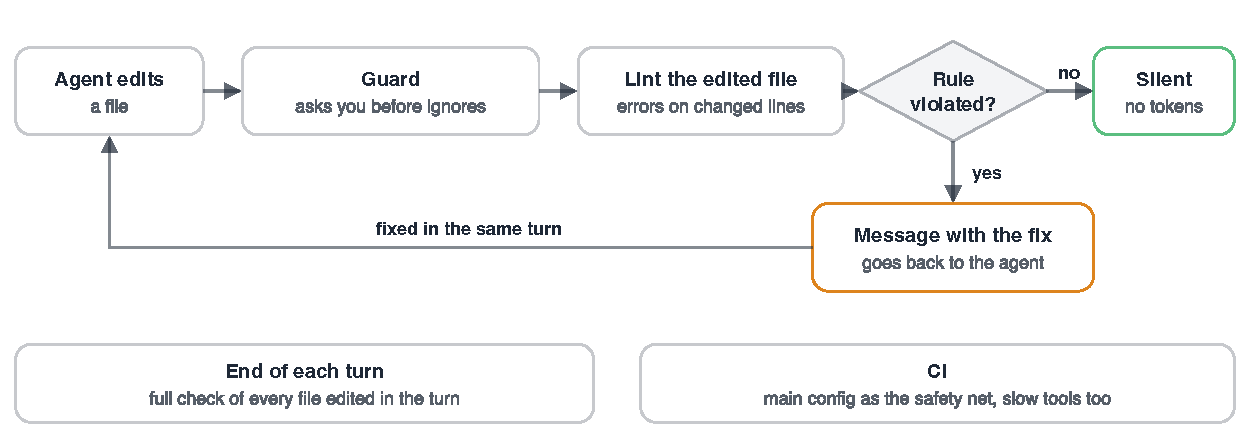
\includegraphics[width=\linewidth]{generated/fig2-loop.pdf}
\caption{The in-session feedback loop of the \arm{rules} arm. After each edit, a guard and the linter run on the edited file. A clean result costs no tokens. A violation returns a message with the fix, and the agent usually fixes it in the same turn. A full check runs at the end of each turn.}
\label{fig:loop}
\end{figure}


We separate two kinds of rules.
A \emph{mechanical} rule changes one expression, for example \texttt{status.HTTP\_404\_NOT\_FOUND} instead of \texttt{status\_code=404}.
A \emph{design-shaping} rule changes where code goes, for example a success notification in the mutation hook instead of in the component.
A mechanical rule is cheap to fix late.
A design-shaping rule is not: a late fix means that the agent must move code that it already wrote.
The pointer exists for this second kind, because it tells the agent the right shape before it writes.

The \arm{rules} arm is the setup that the open-source tool codemyrules installs.
The author of this paper also wrote codemyrules (see the conflict-of-interest statement).

\section{Method}
\label{sec:method}

\subsection{Harness}

agent-rules-bench has four steps (Figure~\ref{fig:bench}).
\textbf{prepare} clones the repository once per arm at the pinned commit, runs the setup script of the arm, and tags the result.
\textbf{run} resets the copy before every session and starts one headless agent session.
For Claude Code this is \texttt{claude -p} with project settings only, so the personal hooks and plugins of the experimenter have no effect.
The study sets the model, the allowed tools and a turn cap of 30.
After each session the harness runs the checkers of the study on the lines that the agent added.
The checkers are the same for every arm and live outside the copies, so no arm is measured with its own rules.
If a run violated a rule, one more session gives the agent precise review feedback, with the same text in every arm.
\textbf{verify} applies the final diff of each run to a clean checkout of the pinned commit, without the setup of any arm, and runs the build and the tests of the project.
\textbf{summarize}, \textbf{compare} and \textbf{pool} produce the statistics.
The harness needs only Node.js and git, and its own test suite runs against a fake agent.

\begin{figure}[H]
\centering
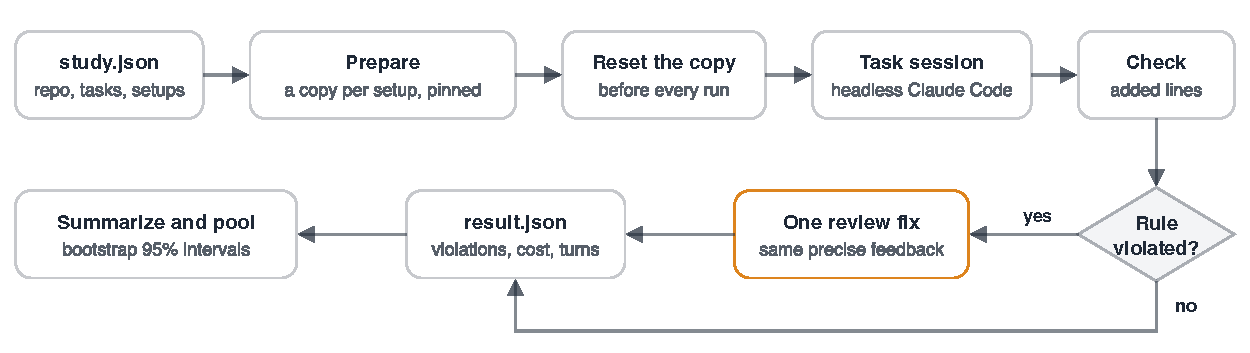
\includegraphics[width=\linewidth]{generated/fig3-bench.pdf}
\caption{One run in agent-rules-bench. Every session starts from a fresh copy of its arm. A run that violated a rule gets one review-fix session.}
\label{fig:bench}
\end{figure}

\subsection{Projects, rules and tasks}

Table~\ref{tab:projects} lists the three public projects.
In each project the existing code already violates the rules: jhipster calls \texttt{Instant.now()} 7 times, the FastAPI routes call the database session 32 times, and all 7 bulletproof-react feature components with a mutation call the notification hook themselves.
An agent that copies nearby code therefore violates the rule.
We chose this design on purpose, because it makes a missed rule visible.
It also means that our violation rates are an upper bound for everyday work (Section~\ref{sec:threats}).

\begin{table}[H]
\centering
\small
\caption{Projects and rules. D = design-shaping, M = mechanical.}
\label{tab:projects}
\begin{tabularx}{\linewidth}{@{}lLL@{}}
\toprule
Project (language, checker) & Rules & Tasks \\
\midrule
jhipster-sample-app (Java, ast-grep) & D: inject a \texttt{Clock}, no \texttt{Instant.now()}. M: authorities from constants, no \texttt{"ROLE\_ADMIN"}. & Admin-only endpoints over the last 7 and 30 days. \\
full-stack-fastapi-template (Python, ast-grep) & D: database access only in \file{crud.py}. M: status-code constants, no integer literals. & Per-user item statistics; clear an item's description with owner checks. \\
bulletproof-react (TypeScript, ESLint) & D: success notifications in the mutation hook. M: query keys from query options. Plans 4--5: 40 conventions. & Edit a comment; change a user's role; rename a team; create teams; four tasks outside all conventions. \\
\bottomrule
\end{tabularx}
\end{table}


Plans 4 and 5 use a list of 40 conventions for bulletproof-react.
The conventions cover architecture, the API layer, authorization, UI, routing, TypeScript, files and the mock API.
Each convention has one prose line, and the same line is its lint message and the text of its review fix.
Prose and lint rule therefore state each convention in the same words.

\subsection{Measures}

A \emph{violation} is a checker finding on an added line in production code, after the task session and before any review fix.
A run is \emph{violating} if it has at least one violation.
\emph{Cost} is the total cost per run that Claude Code reports: the task session plus the review fix, if there was one.
Cost combines tokens, turns, cache use and rework in one number.
We also record turns, tokens, wall time, loop catches, the violations left at the end and the verify result.

\subsection{Models and agents}

All Claude Code runs use \texttt{claude-sonnet-5-5} and \texttt{claude-haiku-5-5}.
We read the model identifiers from the session output.
The runs took place between 1 and 5 November 2026, and the \NClaudeRuns{} runs cost \TotalCost{} in total.

One exploratory study repeats a comparison with a local model, \texttt{qwen3.6:35b-a3b} (Q4\_K\_M quantization), in two other agents, pi and the Codex CLI, with the same feedback loop.
These runs have a turn cap of 60, because the local model needs more turns than the Claude models.
A local model reports no cost, so for these runs we report violations and turns only.

\subsection{Exploratory and pre-registered studies}

The work has two phases, and we keep them apart in all results.

In the first phase we ran four \emph{exploratory} studies.
They had no fixed analysis plan, because their purpose was to form ideas.
While we ran them, we also completed the harness: the arms, the checkers, the review fix and the measures took their final form in this phase.
These studies gave us the questions that the second phase tests, for example what the loop and the pointer each contribute, and what a large always-loaded file costs.
We report their results as exploratory, and we draw no confirmatory conclusion from them.

In the second phase we tested these ideas.
We wrote five analysis plans, Plans~1 to~5, one for each new study.
We committed each plan to the public repository before the first run of its study~\cite{nosek2018prereg}.
The commit history therefore shows that each plan is older than its data.
This is what we mean by \emph{pre-registered}: we fixed the arms, outcomes, hypotheses and statistical tests of a study before we saw any of its results.
Each plan also lists every later deviation with its date.
Only the hypotheses of these plans are confirmatory (Table~\ref{tab:hyp}).

\subsection{Statistics}

For violations we use the exact conditional Cochran--Mantel--Haenszel test~\cite{mantel1959}, one-sided and stratified by study and model.
With one stratum it is Fisher's exact test.
For cost we use the geometric mean of the per-stratum ratios of mean cost, with a 95\% stratified bootstrap interval (10{,}000 resamples, fixed seed)~\cite{efron1993bootstrap} and a one-sided bootstrap $p$.
Within one plan we correct the hypotheses with Holm's method~\cite{holm1979} at a family-wise $\alpha=0.05$.
Plan~1 is the exception: it tests its two hypotheses separately, as the plan states.
Verify pass rates have exact Clopper--Pearson intervals~\cite{clopper1934}.
A script generates every table and every number in this paper from the published results.

\section{Results}
\label{sec:results}

\subsection{Exploratory studies}

Table~\ref{tab:pooled} pools the four exploratory studies, and Appendix~\ref{app:per} lists each comparison.

\begin{table}[H]
\centering
\small
\caption{Exploratory studies: \arm{rules} against prose. Cost change is rules/prose with a 95\% bootstrap interval; violating = runs with a violation after the task. One FastAPI comparison is excluded, because those Sonnet runs skipped the linked documents and wrote no tests, so they did less work. With it, always-loaded prose vs.\ rules is +10\% ($-$1\% to +22\%) for all models. Violations in jhipster-buried include new test files, which its documents did not cover; in production code only, its prose arms violated the rule in 0/8 (Sonnet) and 3/8 (Haiku) runs, so prose the agent can miss was violated in 11/56 runs.}
\label{tab:pooled}
\begin{tabular}{@{}llcccrr@{}}
\toprule
Rule location & Model & Cells & Prose violating & Rules violating & Cost & 95\% CI \\
\midrule
\rows{generated/pooled.tex}
\bottomrule
\end{tabular}
\end{table}


\paragraph{Prose that the agent can miss.}
When the rule was in linked or buried prose, the agent violated it in \PoolMissProse{} runs.
When the same rule was a lint rule, the agent violated it in none.
The cost change was \PoolMissCost{} (\PoolMissCI), because no run with lint rules needed a review fix.
Haiku missed buried prose more often (13 of 24 runs) than Sonnet (4 of 32).
Almost every violation was of a design-shaping rule, and the agent had copied the violating pattern from nearby code.

\paragraph{Prose that the agent reads.}
When the rule was in a short always-loaded \file{CLAUDE.md}, the agent followed it in all runs, as it did with the lint rule, and at equal cost.
A short document behind one clear link was also followed in every run (jhipster, 8 of 8).
Prose therefore fails when it is buried among other text, not because it is prose.

\paragraph{A side effect of always-loaded rules.}
With the rules in \file{CLAUDE.md}, Sonnet on FastAPI stopped opening the linked documents.
It then wrote no tests in any run, so it missed the testing convention that only those documents state.
Always-loaded text can change what else the agent reads.

\subsection{Pre-registered studies}

The five pre-registered studies test the ideas that the exploratory studies gave us.
Table~\ref{tab:hyp} gives every pre-registered hypothesis with its result.
Of the nine hypotheses that we could test, three are supported.
H3 has no test by design, and H4 could not be tested.

\begin{table}[H]
\centering
\footnotesize
\setlength{\tabcolsep}{4pt}
\caption{Pre-registered hypotheses. Violations: violating runs in the first arm vs.\ the second. Cost: change with 95\% stratified bootstrap interval. $p$: exact one-sided CMH (violations) or one-sided bootstrap (cost). Verdicts apply Holm's correction within each plan. H3 is descriptive: it gives the runs whose production code passes the original test suite.}
\label{tab:hyp}
\begin{tabularx}{\linewidth}{@{}lcLLlll@{}}
\toprule
& Plan & Claim & Comparison & Result & $p$ & Supported \\
\midrule
\rows{generated/hypotheses.tex}
\bottomrule
\end{tabularx}
\end{table}

We report the other six in full, because a null result here is also information for practice.

\paragraph{What the loop and the pointer do (Plan 1, 144 runs).}
Three arms differ in one part each: the full setup, the setup without the loop (\arm{pointer\_only}), and the setup without the pointer (\arm{rule\_only}).
Without the loop, \HOneBreaks{} runs violated a rule, against \HOneBreaksAgainst{} with it (H1 supported).
All 8 violations were of the mechanical status-code rule on FastAPI.
This rule had no pointer line, so no text stated it at all.
The three design-shaping rules, each with its pointer line, were violated in 0 of 48 runs without the loop.
The measured value of the loop is therefore that it enforces rules that no prose states.

Without the pointer, the loop caught the design-shaping rule \HTwoCatchNoPointer{} times, against \HOneCatchFull{} times with it, and the cost change was \HTwoCost{} (\HTwoCI; H2 supported).
With the pointer, the agent writes the right shape first.
With the loop alone, the agent reaches the same result through rework.

H3 states that functional correctness does not differ between the three arms, and the plan gives it no test.
The production code passed the original test suite in \HThreeNoLoop{} runs without the loop (exact 95\% interval \HThreeNoLoopCI), in \HThreeNoPointer{} runs without the pointer (\HThreeNoPointerCI) and in \HThreeFull{} runs with the full setup (\HThreeFullCI).

\paragraph{Missed rules over a sequence of sessions (Plan 2).}
This plan ran three tasks in a row on the same copy, to test whether a missed rule compounds.
The usage limit of the account stopped \the\numexpr\SeqPlanned-\SeqOk\relax{} of its \SeqPlanned{} sessions, including all Haiku chains.
The complete Sonnet sessions show no violation in either arm (\HFourBreaks{} vs.\ \HFourBreaksAgainst{} in T2 and T3).
These data cannot test the hypothesis, and we report H4 as not tested.
Plan~2 also named a small descriptive study with a stronger model (Claude Opus, 16 runs, no hypothesis).
We dropped it before any of its runs, because it asks how strong a model must be to follow buried prose, which is a different question.
Plan~3 took its place, and the plan records this change with its date.

\paragraph{A large always-loaded file (Plan 3, 64 runs).}
Teams often put all their documents into the always-loaded file.
We put the project's own \file{AGENTS.md} and its nine guides into \file{CLAUDE.md}, which gives 15.7k tokens in every session, with the two rules in the same positions as in \arm{prose\_buried}.
Against lint rules with short documents, the cost change was \HSixCost{} (\HSixCI, $p=\HSixCostP$; H6 supported).
The large file had \HFiveBreaks{} violating runs against \HFiveBreaksAgainst{} (all Haiku, $p=\HFiveBreaksP$; H5 not supported at 16 runs per arm).
The same rule sentence was followed in a short \file{CLAUDE.md} in all 16 runs.

\paragraph{Forty conventions (Plan 4, 96 runs).}
We stated 40 conventions as 40 prose lines in a short always-loaded file (757 words, 1.9k tokens), and compared them with 40 lint rules and 8 pointers.
The result was even: \HSevenBreaks{} vs.\ \HSevenBreaksAgainst{} violating runs ($p=\HSevenBreaksP$) and a cost change of \HEightCost{} (\HEightCI).
Neither hypothesis is supported.

Stating the conventions mattered in either form.
Without them, every run violated at least one convention, and the review fix gave a cost change of \NoneVsProseCost{} (\NoneVsProseCI).
Only 4 of the 40 conventions were ever violated.
The agent followed the other 36 because the code around it already followed them.
In the \arm{rules} arm, the agent wrote a violation in 13 of 32 runs; each time the loop caught it and the agent fixed it in the same session.

\paragraph{Conventions among business context (Plan 5, 288 runs).}
A real \file{CLAUDE.md} also holds product context.
Every arm got 1,328 words of business context, and the prose arm added the 40 lines.
On the feature tasks, prose was violated in \HNineBreaks{} runs and lint rules in \HNineBreaksAgainst{} ($p=\HNineBreaksP$), with a cost change of \HTenCost{} (\HTenCI).
On four tasks outside the scope of every convention, the 1.9k tokens of prose gave a cost change of \HElevenCost{} (\HElevenCI).
H9 to H11 are not supported.
With a warm prompt cache, the measured extra cost of the prose was about 4\% of a short Sonnet session.
This is close to the price that the token counts predict, and it is too small to detect with 64 runs per arm.

\subsection{Descriptive and post hoc comparisons}

Table~\ref{tab:desc} lists the comparisons that the plans name as descriptive.
Two of them matter for the discussion.

\begin{table}[H]
\centering
\footnotesize
\setlength{\tabcolsep}{3pt}
\caption{Comparisons the plans list as descriptive, without hypothesis tests, and one pooling chosen after the results.}
\label{tab:desc}
\begin{tabularx}{\linewidth}{@{}Lllll@{}}
\toprule
Comparison & Arms & Violating & $p$ & Cost [95\% CI] \\
\midrule
\rows{generated/descriptive.tex}
\bottomrule
\end{tabularx}
\end{table}


First, the same rule sentence was followed in the short file and violated in the large file (3 of 16 runs, all Haiku).
This points to dilution, but the difference is not significant.

Second, Plans 4 and 5 together give \PoolFourFiveBreaks{} violating runs with prose against none with lint rules ($p=\PoolFourFiveP$), at equal cost.
We chose this pooling after we saw both results.
It is therefore a reason to run a confirmatory study, and it does not replace one.

\subsection{Functional correctness}

A rule setup must not make the code worse.
\textbf{verify} built and tested the final diff of each run on the plain upstream commit.
The production code passed the original test suite of the project in \NVerifyOk{} of \NClaudeRuns{} runs, and the arms did not differ.
The \NVerifyFail{} failures are type errors and compile errors that are unrelated to the rules; \NVerifyHaikuFail{} of them come from Haiku.

\subsection{Other agents and a local model}

Table~\ref{tab:local} shows \NLocalRuns{} exploratory runs with a local model in pi and Codex.
These agents load only the root \file{AGENTS.md} by themselves and never load a folder-level pointer.
In these runs, \arm{prose\_buried} therefore means documents that the agent must find without help.

\begin{table}[H]
\centering
\small
\caption{Exploratory: a local model (qwen3.6, 35B, quantized) in pi and Codex on bulletproof-react, 8 runs per cell. $p$: one-sided Fisher against \arm{rules}.}
\label{tab:local}
\begin{tabular}{@{}llcrr@{}}
\toprule
Agent & Arm & Violating & $p$ & Mean turns \\
\midrule
\rows{generated/local.tex}
\bottomrule
\end{tabular}
\end{table}


With prose in documents, every run violated the design-shaping rule in both agents.
With lint rules and the loop, pi had no violating run and Codex had one.
The same rule text in the always-loaded \file{AGENTS.md} did not help in pi (8 of 8 runs violating) and helped partly in Codex (3 of 8).
In pi, the \arm{rules} arm needed about half the turns of the prose arms.
These runs show that the feedback loop carries over to other agents.
They say little about local models in general.

\subsection{Rules that the tool builds}

In the main studies we wrote the lint rules by hand.
As a check of the tool, we also ran the rules that codemyrules built by itself from the \arm{prose\_buried} state of three studies.
These generated rules had \GenBreaks{} violating runs in production code.
Against the hand-written rules, the cost change was \GenCost{} (\GenCI).
Part of this difference comes from less work, because these runs wrote tests less often.
This check is not part of the main question.

\section{Discussion}
\label{sec:discussion}

\paragraph{Where prose fails.}
Prose that the agent reads works.
A short always-loaded file and a short document behind one clear link were followed as well as lint rules.
This agrees with \citet{gloaguen2026agentsmd}, who report that agents follow the instructions in context files well.
Prose fails when the agent does not read it: a bullet in the middle of long linked documents, or a document that the agent never opens.
The failures are not random.
They are design-shaping rules for which the existing code shows the wrong pattern, and the weaker model copies that pattern more often.

\paragraph{What the lint rule adds.}
A lint rule does not depend on the attention of the agent.
Of the \NLoopRuns{} Claude Code runs with the feedback loop, \NLoopBroken{} ended the task with a violation in production code.
This guarantee is cheap when the agent already follows the rule, because a passing check sends nothing to the model.
The ablation shows how the two parts share the work.
The loop enforces rules that nobody wrote down.
The pointer prevents the rework that a late catch of a design-shaping rule causes.

\paragraph{What always-loaded prose costs.}
The token price of a short always-loaded file is small: about \$0.006 per 1k tokens per Sonnet session at median turns, and less with a warm cache.
We could not separate 1.9k tokens of prose from noise.
The cost becomes measurable when the file grows: at 15.7k tokens the cost change was \HSixCost{}.
The risk of a missed rule may also grow: the same rule was followed in the short file and violated in 3 of 16 runs with the large one.
This difference is not significant, and \citet{mcmillan2026adherence} finds no effect of file size on adherence, so we do not claim it.

\paragraph{A guideline.}
From these results we suggest four practices:
\begin{enumerate}
\item Put a rule that a linter can check into a lint rule, and run it in an in-session feedback loop, not only in CI.
\item For a design-shaping rule, add a one-line pointer near the code where the rule applies.
\item Keep the always-loaded file short, and link each longer document with one clear sentence.
\item Do not expect the agent to follow a rule in the middle of long documents, above all when the existing code violates it.
\end{enumerate}

\section{Threats to Validity}
\label{sec:threats}

\paragraph{Adversarial tasks.}
We designed the tasks so that an agent that copies nearby code violates a rule.
Our violation rates are therefore an upper bound.
We did not measure how often natural tasks touch the scope of a rule.
Tasks mined from merged pull requests would answer this question.

\paragraph{Few projects and rules.}
We used three projects, and the pre-registered studies after Plan~1 used only one of them.
The author wrote the 40 conventions and the business context from the documents and the code of the project.
Only 4 of the 40 conventions were ever at risk in the tasks.

\paragraph{Sample size.}
Most cells have 8 runs, and the cost varies widely between runs of the same arm.
Several null results (H5, H7, H9) can only exclude large differences.
They are not evidence of equal compliance.

\paragraph{Measurement.}
The checkers define what a violation is, so their blind spots are ours.
In jhipster-buried the checkers also covered test files, which the documents did not.
The exploratory pool counts those violations (17/56 runs, 11/56 in production code only), and all later studies count production code only.
The harness counts how often the loop reported a finding, but it does not record whether each finding was correct.
We therefore did not measure the false-positive rate of the lint rules.
The review fix is idealised: one precise prompt, no human time and no CI round trip.
Real review costs more, which would favour arms with fewer violations.

\paragraph{Models and agents.}
We used two Claude models in Claude Code and one local model in two other agents, in the versions that were current in early November 2026.
We did not record the exact tool versions at run time.
Updates of a model or an agent can change the results.
Sessions of one arm ran back to back and shared the prompt cache.

\paragraph{Incomplete plan.}
Plan~2 stopped at the usage limit of the account, and we report it as not tested.

\paragraph{Conflict of interest.}
The author wrote codemyrules, which installs the \arm{rules} arm.
To limit this bias, we committed the plans before the runs, we used the same checkers for all arms, we publish every run, and we report the null results of the pre-registered studies in full.

\section{Conclusion}

We compared the places where a coding rule for AI coding agents can live.
Prose works when the agent reads it.
A lint rule with an in-session feedback loop works whether or not the agent reads anything, and it costs nothing while the code is correct.
Lint rules show their clearest gains against prose that the agent can miss and against large always-loaded files.
Against short always-loaded prose, the two come out even in our pre-registered tests.
The harness and all \NAllRuns{} runs are public, so others can test other projects, rules and agents.

\section*{Data and Code Availability}
The harness, all study setups, analysis plans, prompts, session results, diffs and logs are at \url{https://github.com/clirimajeti/agent-rules-bench}.
The command \texttt{node paper/tables.mjs} regenerates every table and every number in this paper from the published results.

\section*{Conflict of Interest}
The author is the developer of codemyrules (\url{https://github.com/clirimajeti/codemyrules}), an open-source, MIT-licensed tool that installs the \arm{rules} arm.
The author receives no income from it.
This work had no external funding.

\section*{Use of AI Assistance}
The author used Claude (Anthropic) for programming assistance and to draft and edit the text of this paper.
The author reviewed all code, analyses and text, and is responsible for the content.

\bibliographystyle{plainnat}
\bibliography{refs}

\appendix
\section{Exploratory Comparisons}
\label{app:per}

\begin{table}[H]
\centering
\footnotesize
\setlength{\tabcolsep}{2.4pt}
\caption{Each exploratory comparison of a prose arm against \arm{rules} (cost = rules/prose).}
\begin{tabular}{@{}lllccrr@{}}
\toprule
Study & Model & Prose arm & Prose violating & Rules violating & Cost & 95\% CI \\
\midrule
\rows{generated/pooled-per-comparison.tex}
\bottomrule
\end{tabular}
\end{table}

\end{document}
